\documentclass{beamer}
\usepackage[utf8]{inputenc}
\usepackage[czech]{babel}
\usepackage{graphicx}
\usepackage{listings}
\usepackage{multicol}
\usepackage{multirow}
\usepackage{algorithm}
\usepackage{algorithmic}
\usepackage{caption}
\usepackage{amsfonts}
\usepackage{amssymb}
\usepackage{amsmath}
\usetheme{Frankfurt}

\title{Shongo}
\subtitle{Reservation system for video and web conferences}
\author{Martin Šrom, Petr Holub, Onřej Pavelka}
\date{November 25, 2013}
\institute{

\includegraphics[width=0.3\textwidth]{cesnet.pdf}
}

% Algorithm
\newcommand{\algf}{\fontsize{2.5mm}{2.5mm}\selectfont}
\newcommand{\algc}[1]{\algf\textbf{#1}}
\algsetup{linenosize=\algf}

% Listings
\lstset{
  basicstyle=\ttfamily\scriptsize,
  keywordstyle=[1]{\textbf},
  morekeywords=[1]{begin,end,if,then,endif},
}

\beamertemplatenavigationsymbolsempty

\begin{document}

\begin{frame}
  \titlepage
\end{frame}

\section{Shongo}\subsection{}
\begin{frame}
  \frametitle{Shongo}
  \textbf{Shongo}
  \begin{itemize}
    \item Reservation system for video/web conferencing resources
    \item Management of resources (e.g., multipoint devices)
    \item Booking of resources (for time slot), e.g.
    \begin{itemize}
      \item virtual room
      \item endpoint      
      \item compartment -- endpoints interconnected by virtual room(s)   
      \item lecture room  
    \end{itemize}
    \item Execution of booked resources, e.g.
    \begin{itemize}
      \item create/delete a virtual room
      \item dial an endpoint
    \end{itemize}    
  \end{itemize}
\end{frame}

\begin{frame}
  \frametitle{Shongo -- Components}
  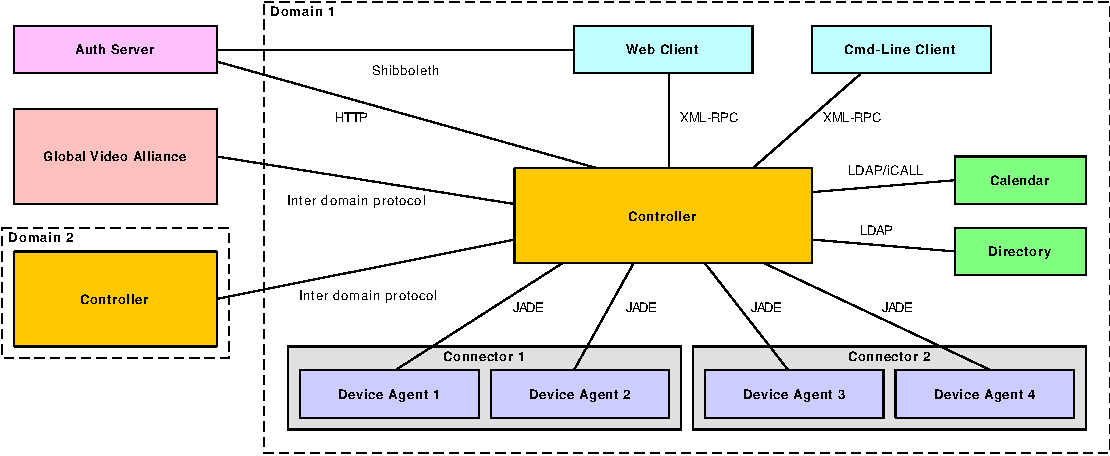
\includegraphics[width=\textwidth]{../architecture/diagrams/dd_architecture.pdf}
\end{frame}

\begin{frame}
  \frametitle{Shongo -- Implemented Components}
  \begin{itemize}
    \item Auth Server (PHP)
    \item Single Domain
    \begin{itemize}
      \item Domain Controller (Java)
      \item Connector Agents for devices (Java)
      \item Web Interface (Java)
      \item Cmd-Line Client (Perl)
    \end{itemize}
  \end{itemize}
  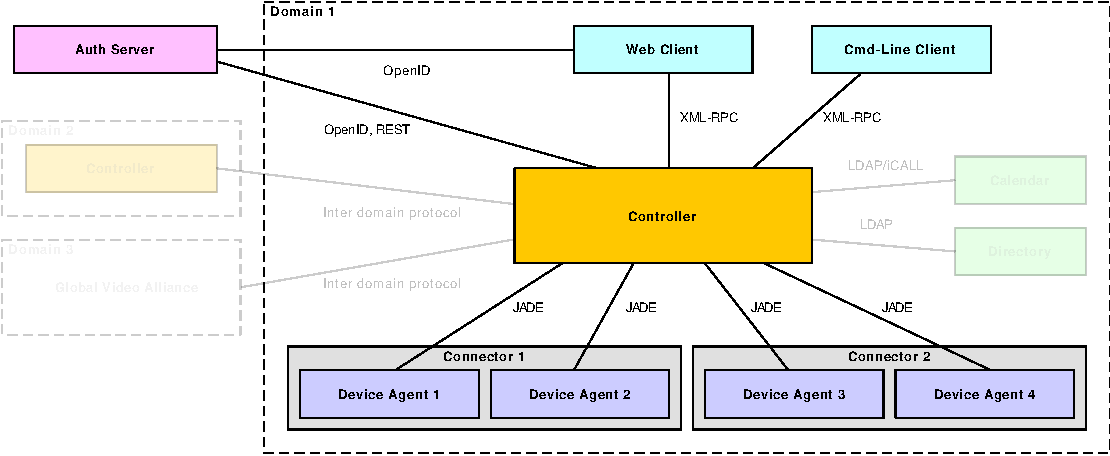
\includegraphics[width=\textwidth]{../architecture/diagrams/dd_architecture_implemented.pdf}
\end{frame}

\begin{frame}
  \frametitle{Shongo}
  \textbf{Currently}
  \begin{itemize}
    \item Booking, execution and management of virtual rooms in multipoint devices
    \item H.323/SIP (Cisco MCU) and Adobe Connect
    \item Single domain
  \end{itemize}
  \textbf{In development}
  \begin{itemize}
    \item Recording of virtual rooms (Cisco TCS)
    \item Merging multiple user identities
  \end{itemize}
  \textbf{Future}
  \begin{itemize}
    \item Booking of seminar rooms in Adobe Connect
    \item Streaming of virtual rooms
    \item Multiple domains (inter-domain booking protocol)
  \end{itemize}
\end{frame}

\section{Web Interface -- Demo}\subsection{}

\begin{frame}
  \frametitle{Web Interface -- Demo}
  \begin{itemize}
    \item Show log-in
      \begin{itemize}
        \item Hostel registration    
      \end{itemize}
    \item Show dashboard
      \begin{itemize}
        \item Ad-hoc room
        \item Permanent room and capacities
      \end{itemize}
    \item User settings (time zone, language)      
    \item Create ad-hoc/permanent room/capacity
      \begin{itemize}
        \item Configuration of user roles
        \item Configuration of participants (for Adobe Connect)
        \item Email notifications
      \end{itemize}        
    \item Room management
      \begin{itemize}
        \item Active participants
        \item Room layout
      \end{itemize}    
    \item List of reservation requests
    \item Detail of reservation request
      \begin{itemize}
        \item Modify the reservation request
        \item History of the reservation request        
      \end{itemize}          
  \end{itemize}
\end{frame}

\end{document}